\documentclass{article}
\usepackage[utf8]{inputenc}
\usepackage[margin=1in]{geometry}
\usepackage{hyperref}
\usepackage{graphicx}
\usepackage{float}

\title{Interpolation on Lincoln Weather}
\author{Khang Phan}
\date{December 2018}

\begin{document}

\maketitle
\clearpage

\tableofcontents
\listoffigures
\clearpage

\section{Introduction}
\section{Data}
The data is collected from \href{https://www.ncdc.noaa.gov/}{National Climatic Data Center}. It contains information in several data station across Nebraska from January 2010 to 2018. For the investigation, we use the data in 2011 at station USW00014939, which has 366 data points.
\section{Interpolation Method}
In this investigation, we measure four different interpolation method: Linear Spline, Quadratic Spline, Cubic Spline, and Best Fit Polynomial. 
\subsection{Linear Spline}
\begin{figure}[H]
    \centering
    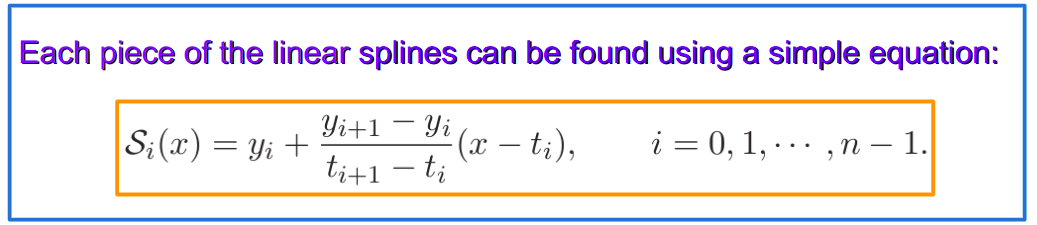
\includegraphics[width=500pt]{Linear}
    \caption{Linear Spline}
    \label{fig:my_label}
\end{figure}
\subsection{Quadratic Spline}
\begin{figure}[H]
    \centering
    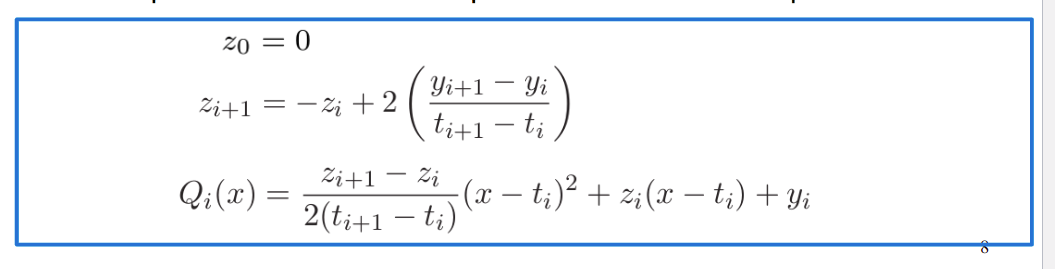
\includegraphics[width=500pt]{quadratic}
    \caption{Quadratic Spline}
    \label{fig:my_label}
\end{figure}
\subsection{Cubic Spline}
\begin{figure}[H]
    \centering
    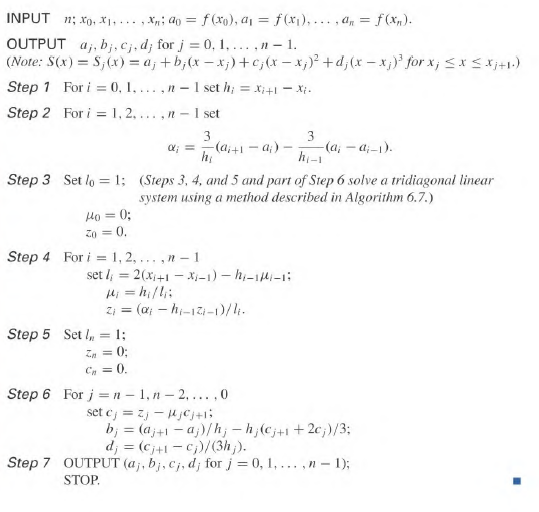
\includegraphics{cubic}
    \caption{Cublic Spline}
\end{figure}
\subsection{Best Fit Polynomial}
Polynomial function: $$f(x) = \sum_{i=0}^{k} a_{i}x^i = a_0 + ... + a_k*x^k$$\\
Optimize function: $$error = \sum_{i=1}^{n} (y_i-f(x_i))^2$$
\section{Experiment}
\subsection{Sampling method}
We ramdomly select sets of points to use as input for our interpolation methods. Other points are used to measure the accuracy. The sets always contain the data on January 1, 2011 and January 1, 2012, so all missing points are in the range. The size of the sets include 330, 300, 270, 240, 73, and 37.
\subsection{Graph}
Following are the graph of different methods used on a set of input sized 270. The green line indicates the actual data, and the red line is my predicted function.\\
The first three graphs are Linear Spline, Quadratic Spline, and Cubic Spline respectively. From the graph, we can see clearly Quadratic Spline does not work in this case. It goes far above the below the actual data points. On the other hand, Cubic Spline and Linear Spline are much more accurate. They are much closer to the actual data. Also, they are visually similar to each other.\\
\begin{figure}[H]
    \centering
    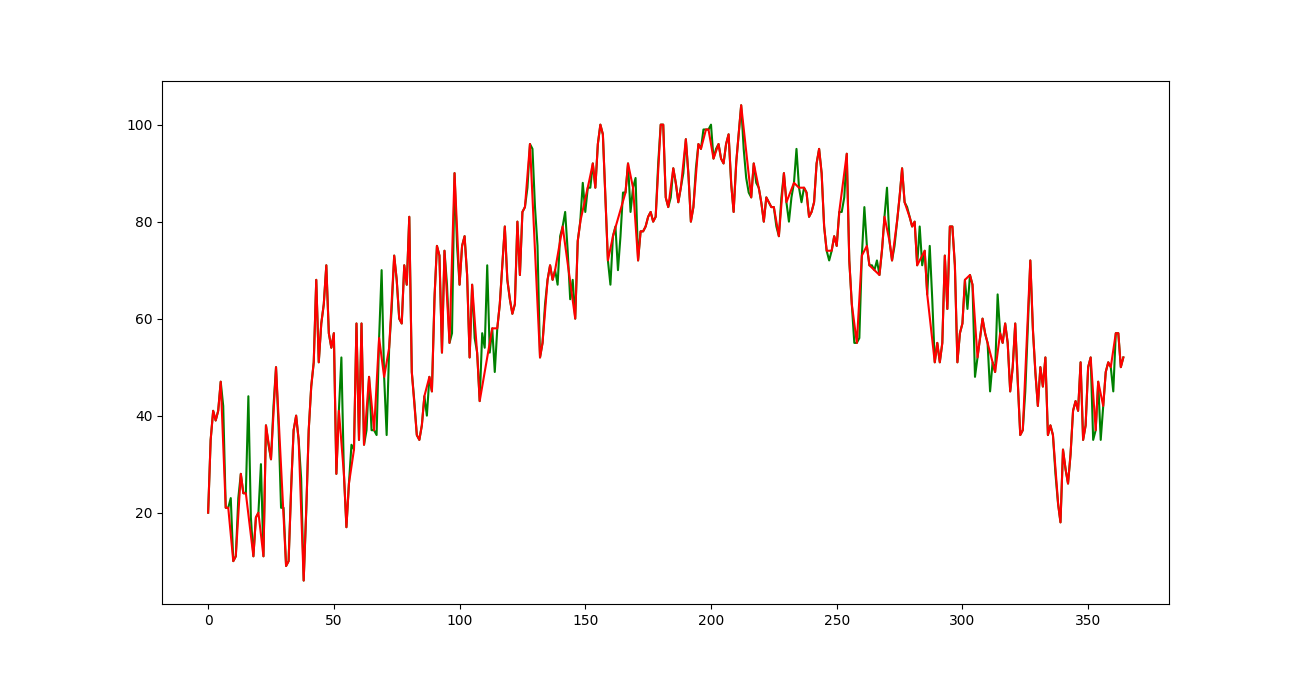
\includegraphics[height=200pt]{linear_spline_270.png}    
    \caption{Linear Spline}
    \label{linear spline}
\end{figure}
\begin{figure}[H]
    \centering
    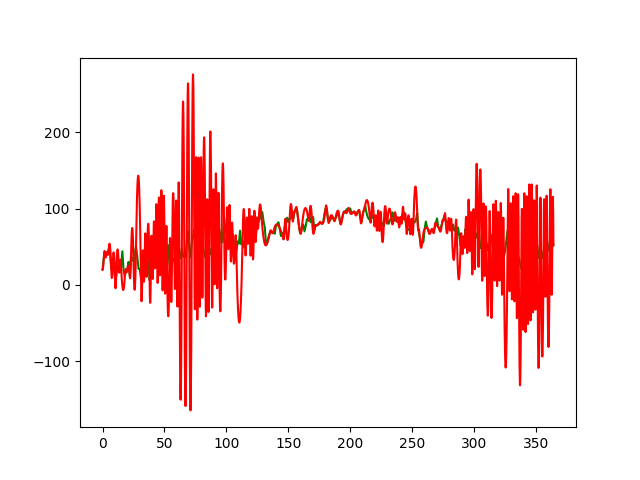
\includegraphics[height=200pt]{quadratic_spline_270.png}    
    \caption{Quadratic Spline}
    \label{quadratic spline}
\end{figure}
\begin{figure}[H]
    \centering
    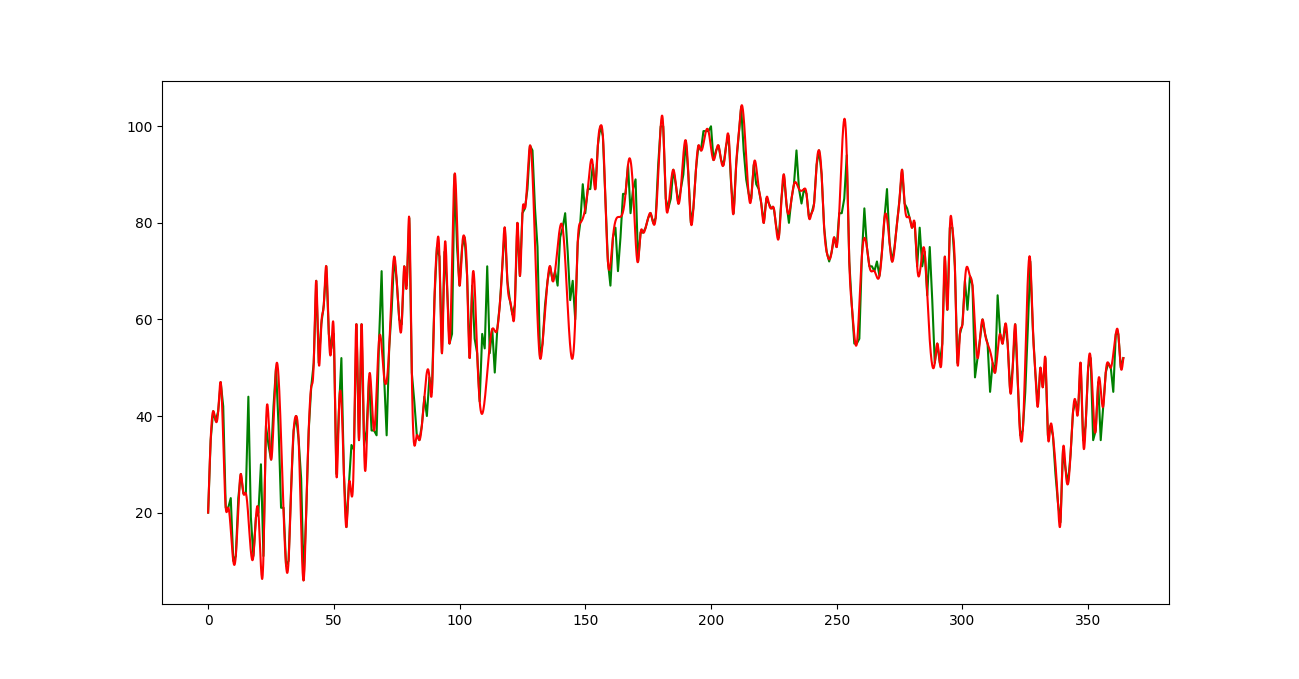
\includegraphics[height=200pt]{cubic_spline_270.png}
    \caption{Cubic Spline}
    \label{cubic spline}
\end{figure}
Next figures are graphs of degree one to nine polynomials having smallest sum of square errors. The figures give us the trend of temperature. From the curves, we have some idea when the temperature should go up or down. From the graphs, we can see the difference between linear function and the rest. When comparing polynomial degree two to nine, we could not see big changes between any two consecutive functions. \\
\begin{figure}[H]
    \centering
    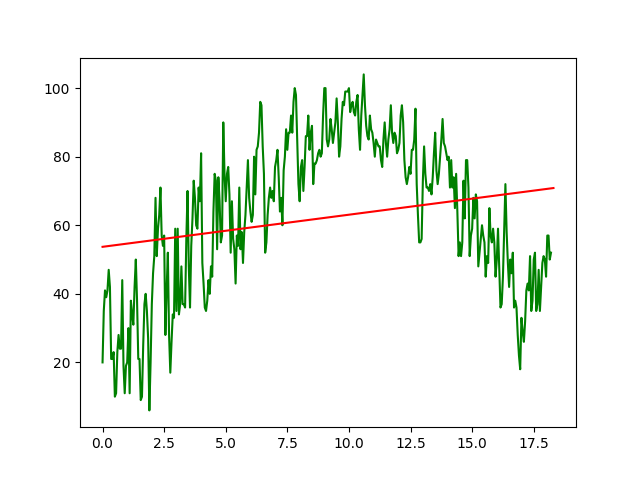
\includegraphics[height=200pt]{1poly_270.png}
    \caption{Degree one polynomial}
\end{figure}
\begin{figure}[H]
    \centering
    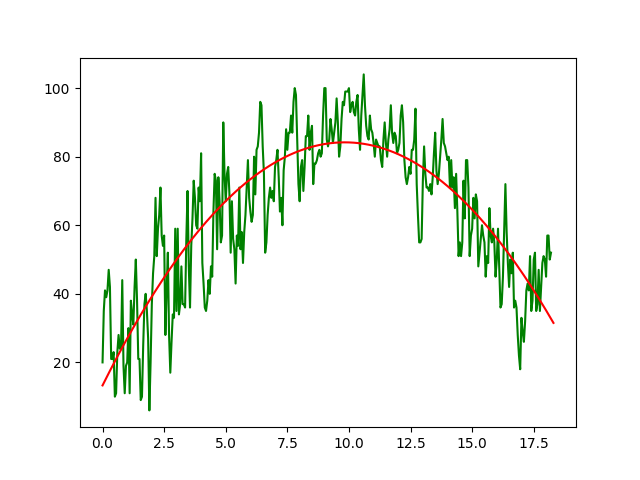
\includegraphics[height=200pt]{2poly_270.png}
    \caption{Degree two polynomial}
\end{figure}
\begin{figure}[H]
    \centering
    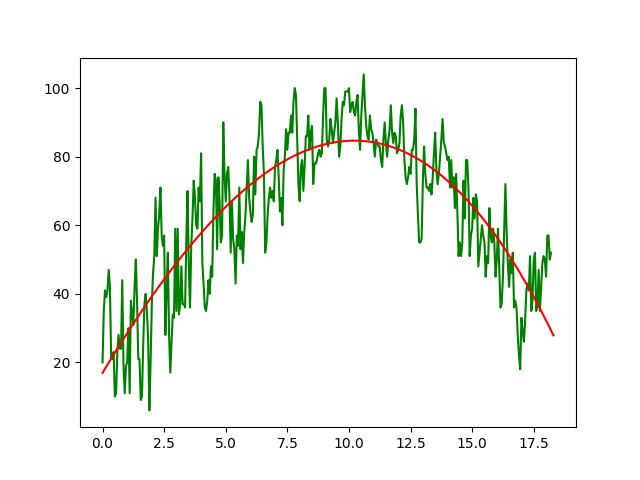
\includegraphics[height=200pt]{3poly_270.png}
    \caption{Degree three polynomial}
\end{figure}
\begin{figure}[H]
    \centering
    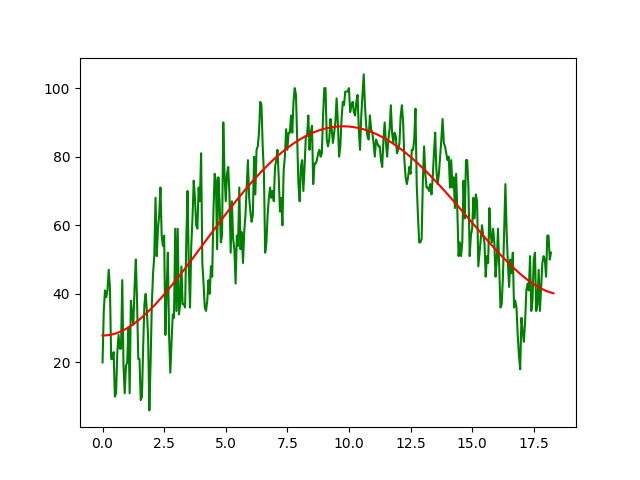
\includegraphics[height=200pt]{4poly_270.png}
    \caption{Degree four polynomial}
\end{figure}
\begin{figure}[H]
    \centering
    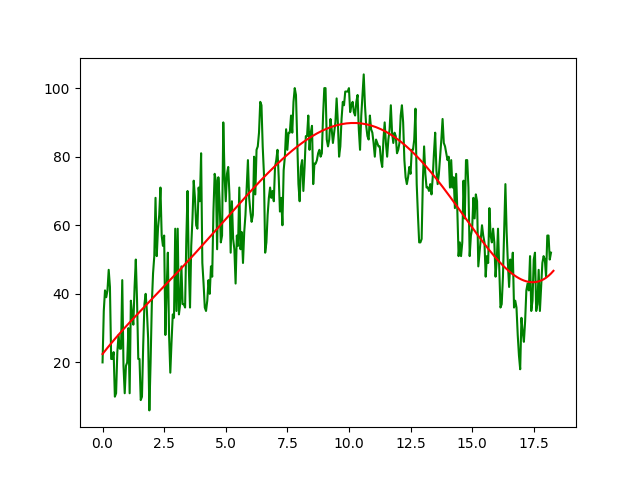
\includegraphics[height=200pt]{5poly_270.png}
    \caption{Degree five polynomial}
\end{figure}
\begin{figure}[H]
    \centering
    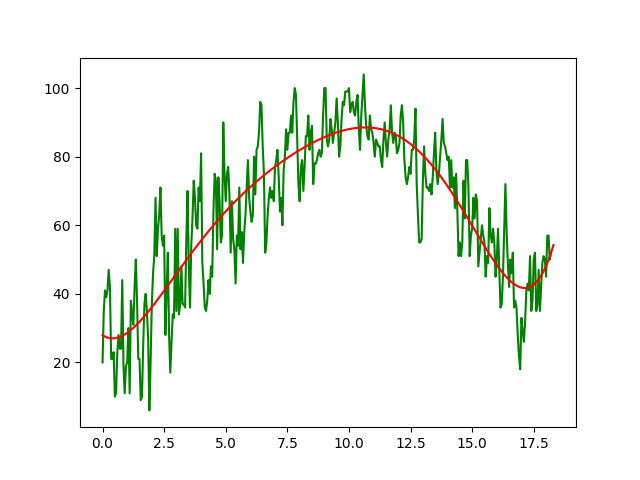
\includegraphics[height=200pt]{6poly_270.png}
    \caption{Degree six polynomial}
\end{figure}
\begin{figure}[H]
    \centering
    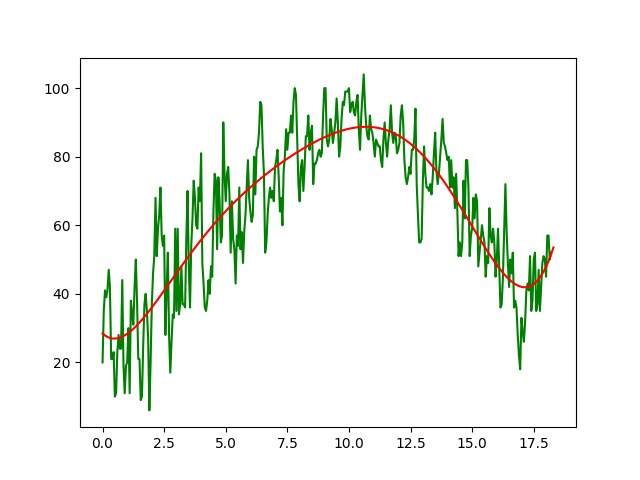
\includegraphics[height=200pt]{7poly_270.png}
    \caption{Degree seven polynomial}
\end{figure}
\begin{figure}[H]
    \centering
    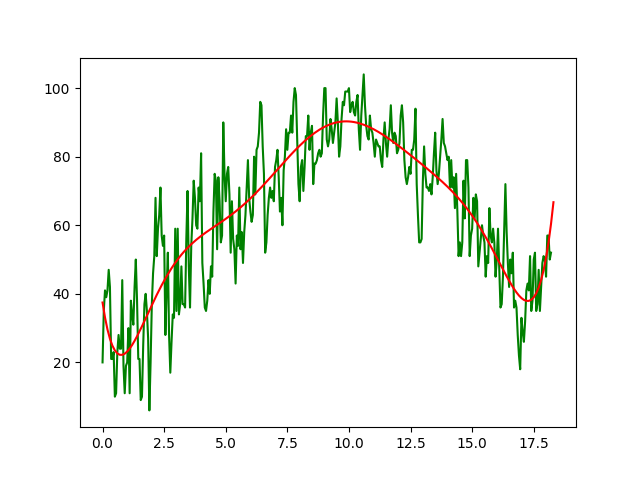
\includegraphics[height=200pt]{8poly_270.png}
    \caption{Degree eight polynomial}
\end{figure}
\begin{figure}[H]
    \centering
    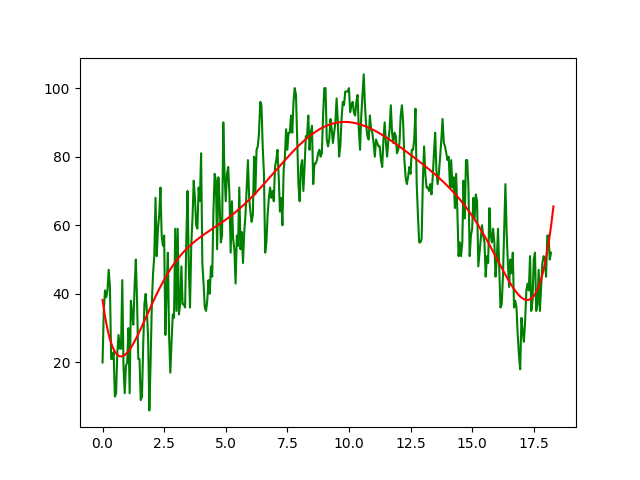
\includegraphics[height=200pt]{9poly_270.png}
    \caption{Degree nine polynomial}
\end{figure}

\subsection{Aggregation}
To compare the accuracy of above methods, we randomly sample data points and run interpolations on them. Then we use the mean of square errors to determine their accuracy. Figure \ref{aggregate} shows the results after 100 runs of each size. We can see, for each method (i.e. each column), as the sample size decreases, the errors increases. \\
Comparing the piecewise interpolation, Quadratic Spline error is significantly larger then Linear or Cubic. Linear Spline and Cubic Spline is very similar, as we can see from above graph; as Linear seems to be a little better. Comparing polynomials, linear has much higher errors, while other degree from two to nine are close. As degree gets higher, the error rates decrease. We also notice that as the sample size decreases, error terms of Piecewise interpolation method increases much faster than Polynomial functions.

\begin{figure}[H]
    \centering
    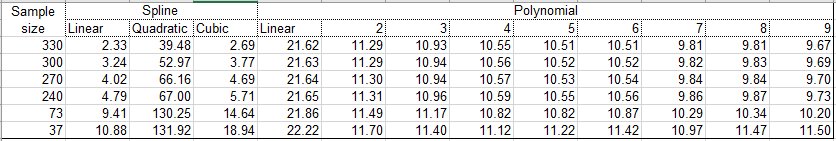
\includegraphics[width=500pt]{Capture}
    \caption{Result}
    \label{aggregate}
\end{figure}

\section{Conclusion}
After the experiments, our first impression is that Linear Spline seems to be the best method in general. Cubic Spline would also work very well, but it requires more complex implementation. When the sample size is small, we can use Polynomial functions, as they give us information about the temperature trend with accuracy comparable of Linear/Cubic Spline give.

\section{Reference}


\end{document}
